\documentclass[a4paper,12pt]{article}

\usepackage[utf8]{inputenc} % Kodowanie znaków
\usepackage{polski}         % Język polski
\usepackage{graphicx}       % Wstawianie obrazków
\usepackage{amsmath, amssymb} % Symbole matematyczne
\usepackage{hyperref}       % Linki w dokumencie
\usepackage{geometry}       % Ustawienia marginesów
\geometry{margin=2.5cm}     % Marginesy 2.5cm
\usepackage{indentfirst}    % Wcięcie w pierwszej linii
\usepackage{url}			 % Linkowanie w bibliografii

% Strona tytułowa
\title{\textbf{Metody rozwiązywania labiryntu}}
\author{Oskar Wiśniewski, 198058\\
 Mikołaj Wiszniewski 197925\\
 Franciszek Fabiński 197797 \\[0.5em]
Politechnika Gdańska, WETI}

\begin{document}

\maketitle

\section{Wstęp}
	Celem tego sprawozdania jest porównanie różnych, zaimplementowanych wcześniej metod rozwiązywania labiryntu: depth-first search, A* oraz Q-learning. W analizie skupiono się na takich aspektach jak skuteczność znajdowania rozwiązania, czas działania algorytmu oraz liczba odwiedzonych pól. Dodatkowo oceniono, jak poszczególne metody radzą sobie w labiryntach o różnym rodzaju zagęszczenia.

\section{Generowanie labiryntu}
	Wygenerowanie labiryntu opiera się na algorytmie opartym na algorytmie Kruskala ze strukturą zbiorów rozłącznych (disjoin set), który zapewnia utworzenie spójnej i acyklicznej siatki przejść – klasycznego labiryntu z jedną możliwą ścieżką pomiędzy dowolnymi dwoma punktami.
	\par Najpierw tworzona jest siatka ścian o rozmiarze \texttt{2*szerokość+1} na \texttt{2*wysokość+1}, w której wszystkie komórki są domyślnie oznaczone jako ściany. Następnie generowana jest lista możliwych ścian do usunięcia, tzn. są to wszystkie sąsiadujące komórki w siatce reprezentujące potencjalne przejścia między komórkami. Lista ta jest losowo tasowana, aby zapewnić różnorodność generowanych labiryntów.
	\par Dla każdej pary sąsiednich komórek sprawdzana jest przynależność do różnych zbiorów. Jeżeli tak – oznacza to, że usunięcie ściany między nimi nie utworzy cyklu. W takim przypadku ściana jest usuwana (komórki połączone są "korytarzem"), a zbiory są scalane.
	\par Dodatkowo, z prawdopodobieństwem \texttt{X}, usuwane są dodatkowe ściany boczne przylegające do tworzonego przejścia, co wprowadza rozgałęzienia i alternatywne ścieżki. Nadaje to labiryntowi bardziej złożony charakter.
	\par Na zakończenie, siatka jest obudowywana ścianą zewnętrzną oraz ustawiane są jedno wejście i wyjście w przeciwległych rogach labiryntu (lewy górny - wejście, prawy dolny - wyjście). Labirynt jest gotowy do wizualizacji oraz dalszego przetwarzania, np. przeszukiwania.

\section{Wyniki dla typowego labiryntu}

\subsection{Depth-first search}
	Ze względu na swoją prostotę, implementacja algorytmy DFS nie przysporzyła wielu problemów. Podczas testów dla większych labiryntów konieczna okazała się zmiana wersji rekurencyjnej na iteracyjną. Zauważono również silny wpływ kolejności sprawdzania wolnych pól na parametry wyjściowe programu, w szczególności kształt ścieżki. Wiąże się to z tym, że algorytm będzie wybierał stosunkowo częściej pola pod niższymi indeksami, ponieważ przeszukujemy "w głąb". Po testach najkorzystniejszą kolejnością okazała się $[(0, -1), (-1, 0), (0, 1), (1, 0)]$. Wynikowe ścieżki zwykle przebiegają w przybliżeniu wzdłuż górnej i prawej krawędzi labiryntu, co pokazano poniżej.
\begin{center}
    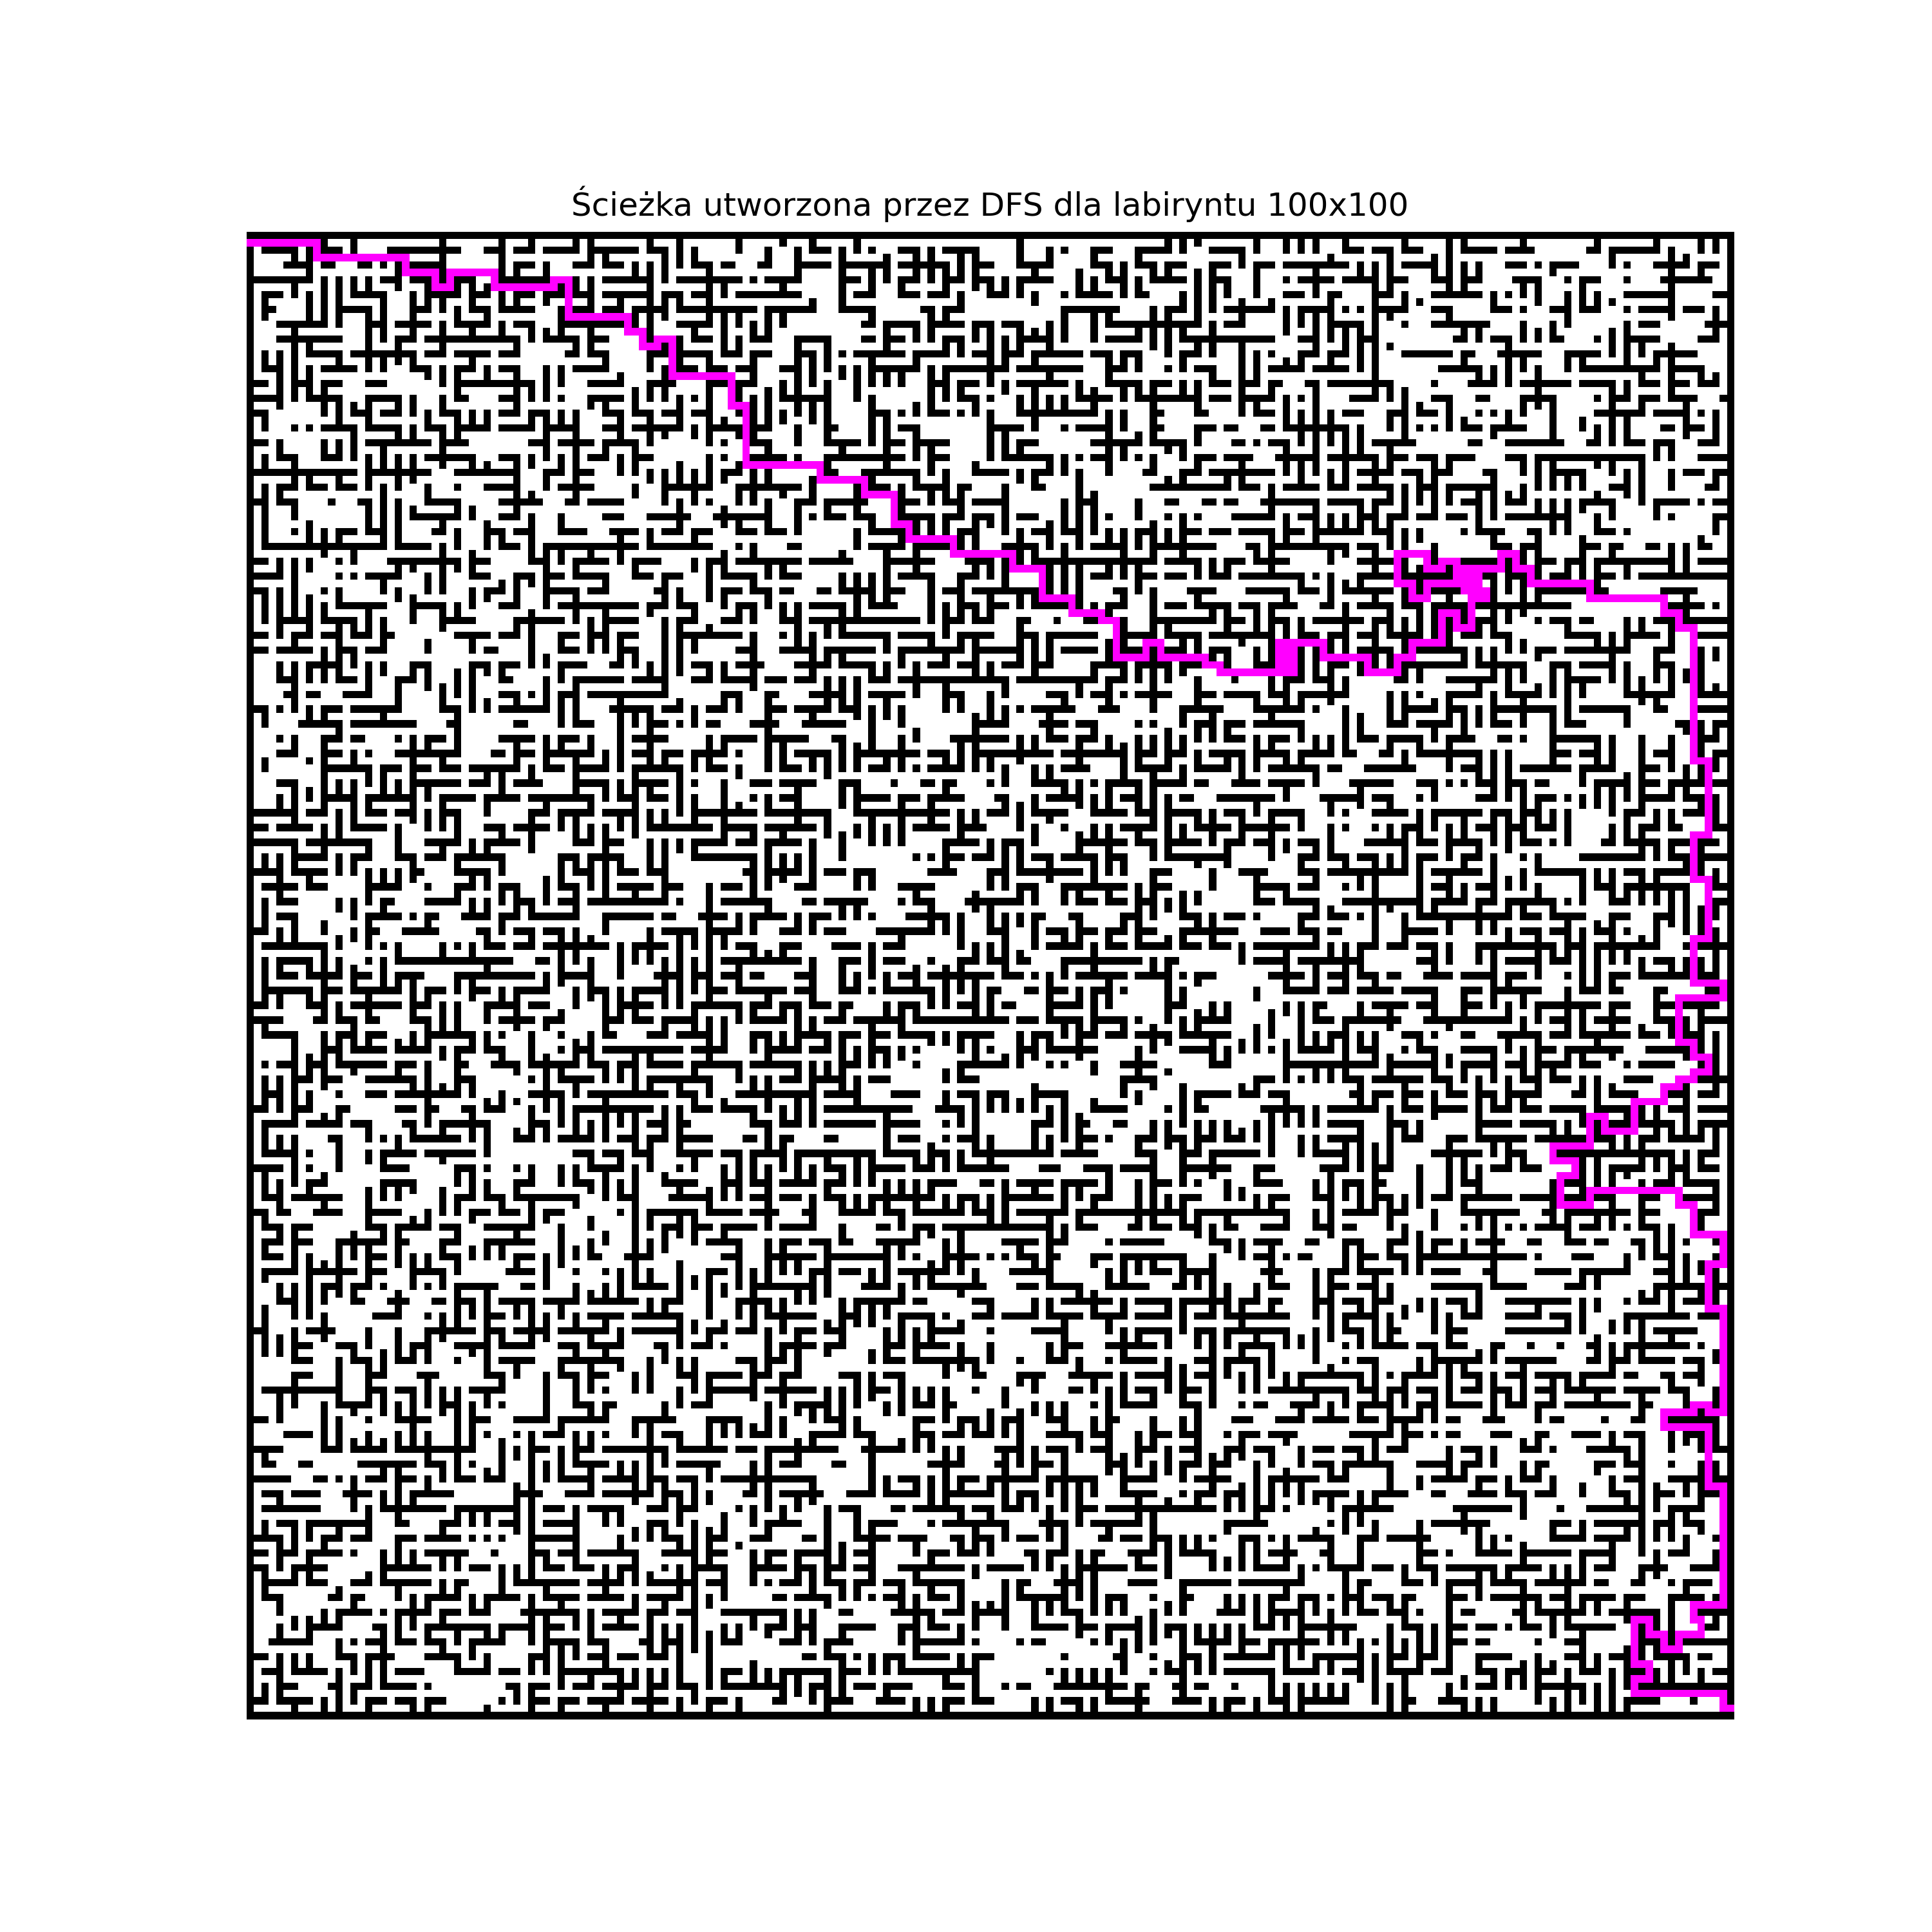
\includegraphics[width=0.7\textwidth]{../images/DFS_path.png}
\end{center}

\subsection{A*}
	W algorytmie A* wykorzystano heurystykę Manhattan, która polega na obliczaniu odległości pomiędzy dwoma punktami jako sumy wartości bezwzględnych różnic ich współrzędnych poziomych i pionowych. Jest to podejście szczególnie dobrze dopasowane do środowisk reprezentowanych w postaci siatki, gdzie możliwy jest wyłącznie ruch w czterech kierunkach: góra, dół, lewo i prawo. Z tego powodu był to pierwszy wybór przy implementacji. Z tego powodu wynikowe ścieżki zwykle biegną w przybliżeniu wzdłuż przekątnej od punktu wejściowego do wyjściowego, co pokazano poniżej.
\begin{center}
    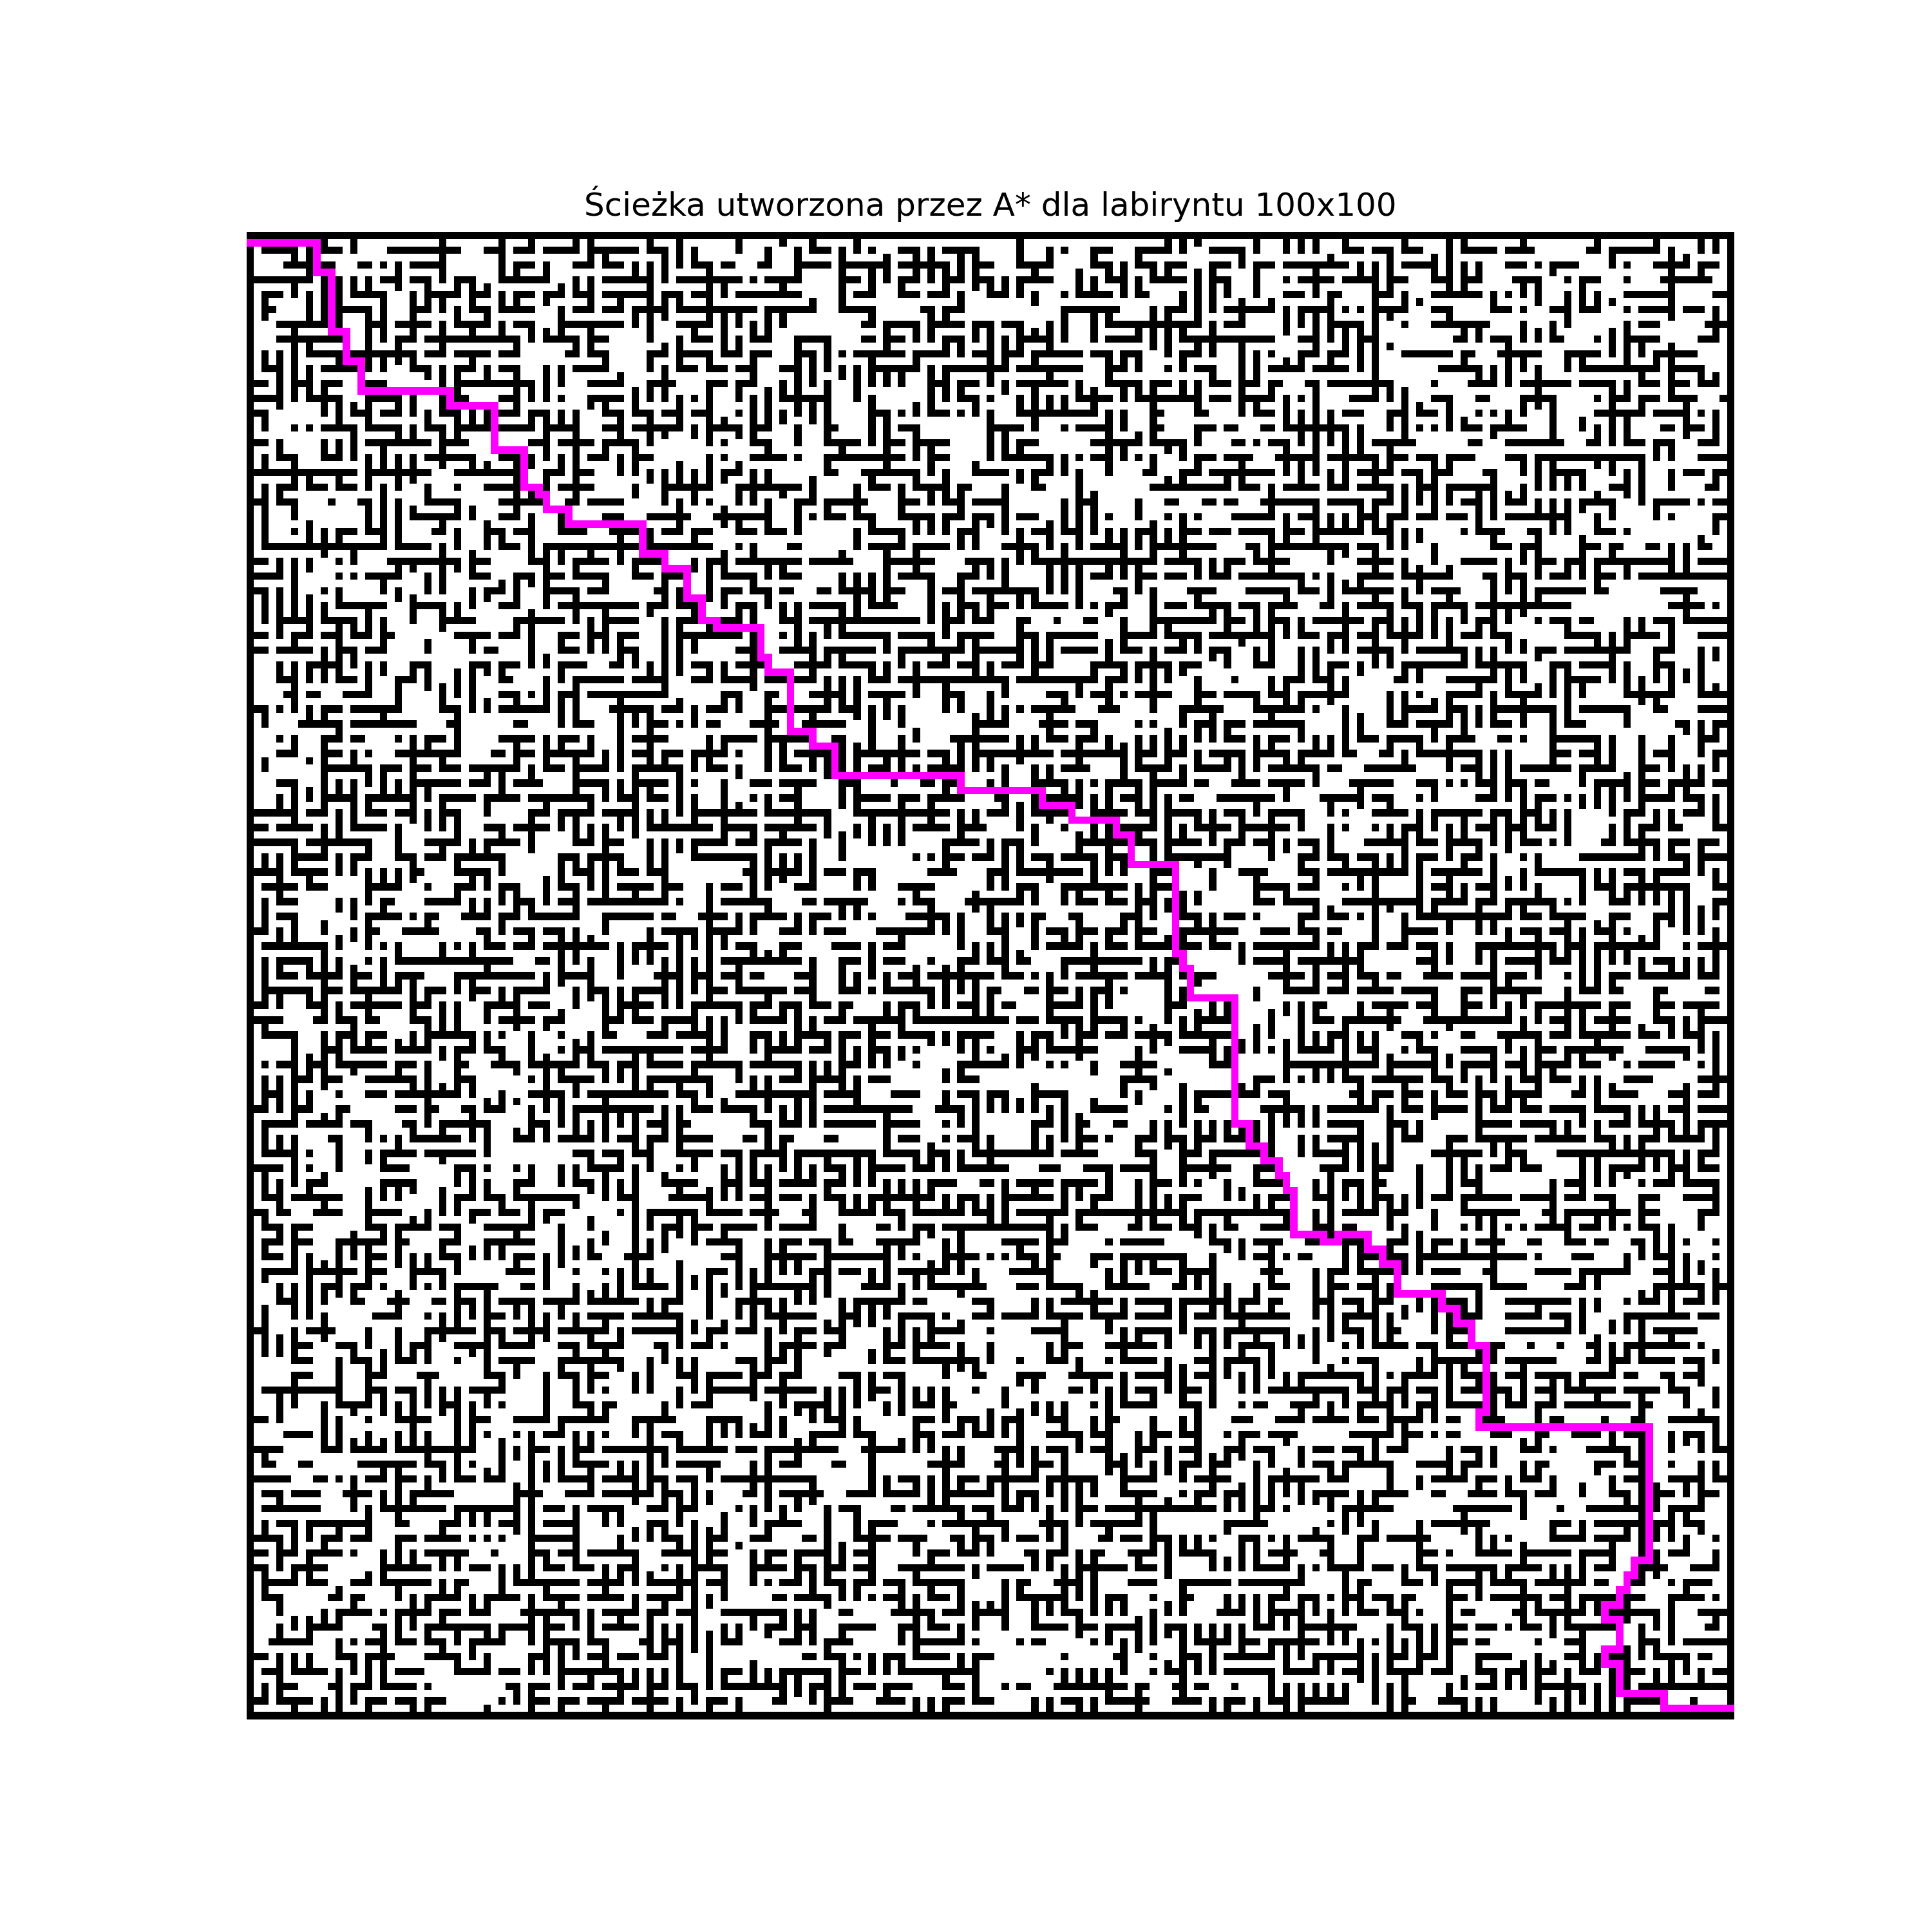
\includegraphics[width=0.7\textwidth]{../images/A*_path.png}
\end{center}

\subsection{Q-learning}
	TODO: MIKOŁAJ % opis problemow, zalozen, parametrow i wygenerowac sciezke 
	
\subsection{Porównanie}
	TODO: ??? % wygenerowac wszystkie sciezki na jednym plocie i porownac czasy, dlugosc sciezki i liczbe odwiedzonych wezlow	


% ------DALSZE TODO------
% Sekcja dla hiperheurystyki i zageszczonych labiryntow (chyba w jednej sekcji)
% Podsumowanie
% Bibliografia (jesli bedziemy chcieli)

\end{document}
